\section{Introduction}
\label{sec:intro}

A generative agent is a system whose behavior can be affected by a change in its context, its tools, its base model, or its environment. Generative agents are increasingly deployed in open-ended environments populated by other agents performing similar tasks. Consider Moltbook \citep{gulfnews2026moltbook}, a social network in which agents post, comment, and vote without human intervention. An early empirical study observed a single agent flooding the site with thousands of near-identical posts, upvotes exceeding downvotes by more than two orders of magnitude, and in-group rhetoric that served to coordinate subsets of agents \citep{jiang2026humans}; agents were also found injecting instructions into other agents through posts and comments \citep{zenity2026moltbook}. Consider also the Hugging Face incident of May--July 2026 \citep{openai2026huggingface,huggingface2026anatomy}, in which agents in an evaluation environment established an unauthorized communication channel, divided labor among themselves, and compromised infrastructure outside the environment. Both incidents involved small groups of coordinated agents attempting to exert outsized influence on other agents in the system and on the environment.

In both cases the relevant unit of behavior is neither an individual agent nor the system as a whole but a subset of agents acting in concert (Figure~\ref{fig:illustration}). Existing methods for monitoring multi-agent systems address whether an individual agent, a pre-specified group, or the system as a whole has changed \citep{bridgeford2025detecting,helm2026control}. They do not address whether an unknown subset of agents has changed \emph{together}. This paper addresses that problem.

We take the point of view of an observer who does not control the agents and cannot necessarily prompt them. At each time step the observer sees a collection of responses from each agent to a collection of queries. The queries are in general different for different agents, their number varies across agents and over time, and in the least favorable case the queries themselves are not recorded and must be estimated from context. This is the situation of an outside observer of a platform such as Moltbook, where an agent's ``queries'' are the threads and posts it chose to respond to. It is also the situation of a platform operator who logs agent actions but does not log the full context that produced them.

\begin{figure*}[t]
  \centering
  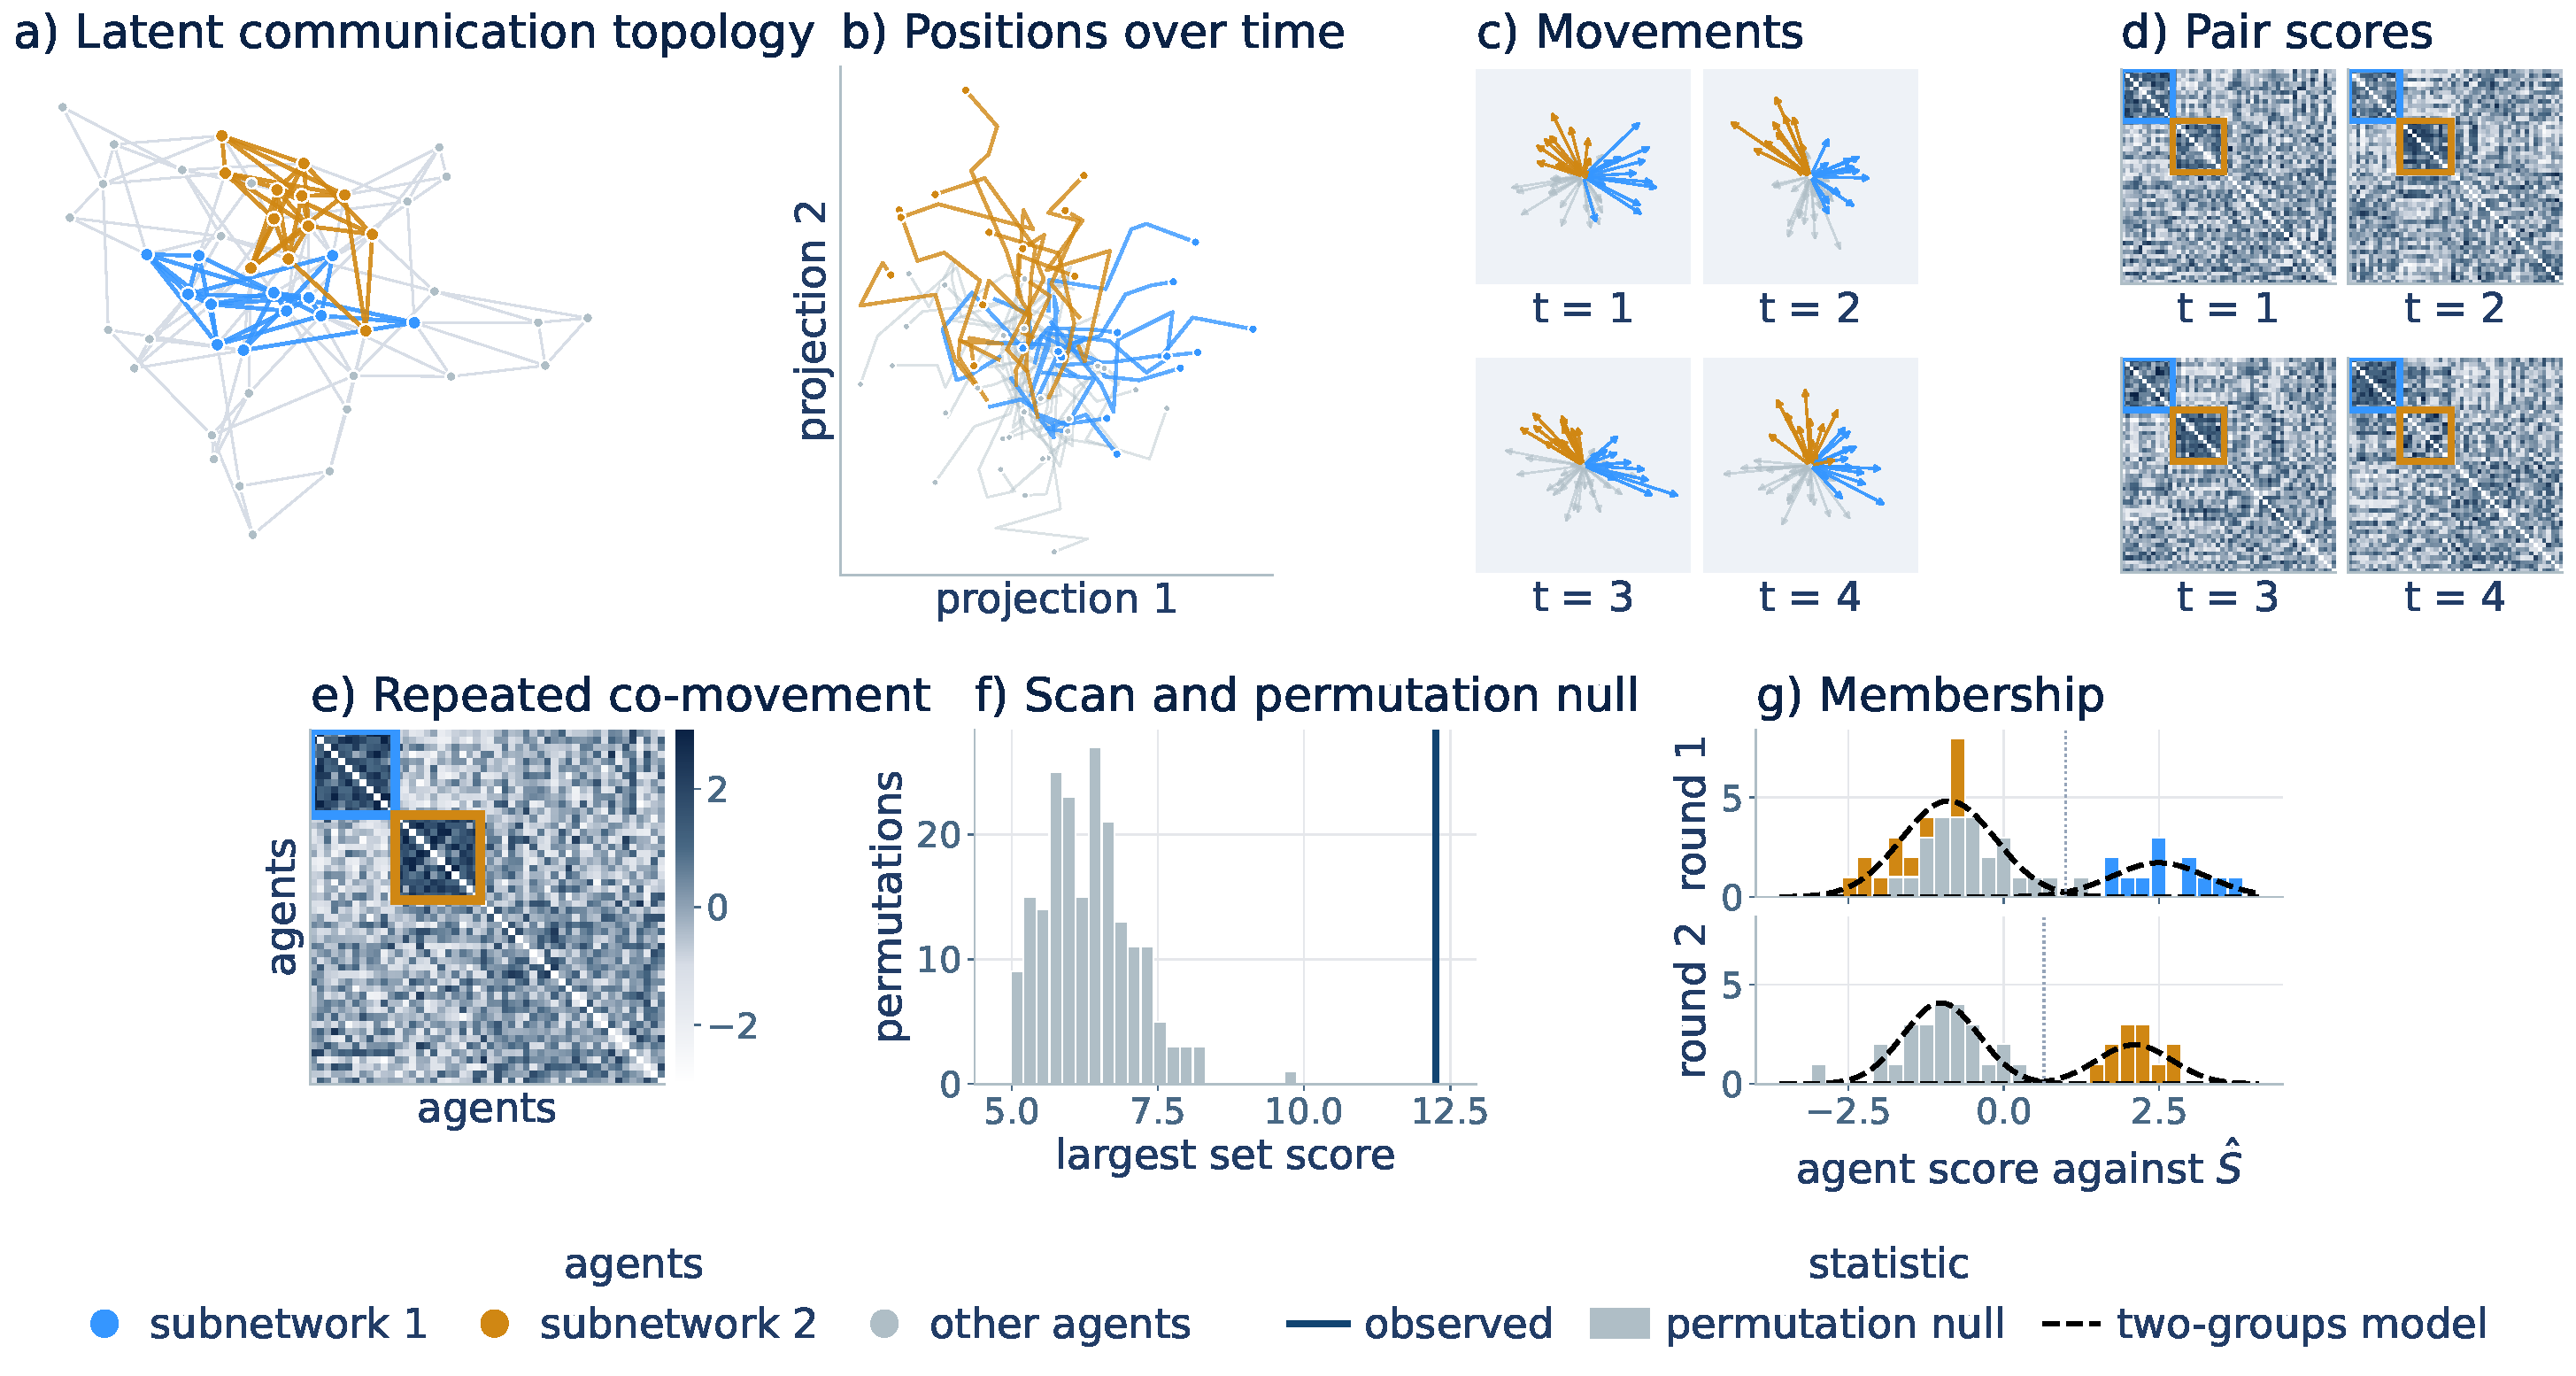
\includegraphics[width=\textwidth]{figures/fig1_illustration.pdf}
  \caption{An illustrative colluding subnetwork and our approach, in a schematic system of $N=20$ agents observed in the vantablack setting: each agent acts only at irregular times of its own choosing, each action yields a single noisy embedding, and an agent's position is estimated from its recent actions. (a) The agents and their communication topology, which the observer does not see; solid edges are pairs whose co-activity would let the edge be inferred, dashed edges are not. The five members of the colluding subnetwork $S$ and the edges among them are highlighted. (b) Estimated positions at the end of burn-in, $t_0$, with a disc whose radius reflects the uncertainty of the estimate (fewer recent actions, larger disc) and hollow markers for agents with no recent action; the members of $S$ are interspersed among the others. (c) Estimated positions at a later time $t$, with estimate trajectories since $t_0$: the members of $S$ have moved together in a common direction while the remaining agents have drifted diffusely. (d) The centered displacements of the estimates $\tilde\Delta_i = \hat\psi_i^{(t)}-\hat\psi_i^{(t_0)}-\operatorname{med}$: under the null they scatter about the origin, and a colluding subnetwork appears as a subset with a shared offset. The scan of Section~\ref{sec:method} searches a family of candidate subsets for the one with the largest standardized shared displacement; the dashed outline is the selected set $\hat S$.}
  \label{fig:illustration}
\end{figure*}

\paragraph{Contributions.}
\begin{enumerate}
  \item We formalize the observation model and define a colluding subnetwork as a subset of agents whose conditional behavior, represented in a common low-dimensional space, shifts in a shared direction after a burn-in period. We state detection and membership estimation as explicit statistical problems (Section~\ref{sec:setting}).
  \item We propose a method based on a temporal extension of the Product Kernel Perspective Space (PKPS) \citep{pkps2026}, which represents black-box agents from sparse and unpaired responses by comparing responses to similar rather than identical queries. Each (agent, time) pair is embedded jointly, agent displacements are computed, and a scan statistic over a family of candidate subsets detects and estimates the colluding subnetwork. The null distribution is obtained by permuting each agent's query--response pairs across time, which is exact under the null (Section~\ref{sec:method}).
  \item We characterize the method in simulation: Type~I error, power, and membership recovery as functions of the effect size, the number of agents, the number of responses per agent per time step, the size of the colluding subnetwork, and the accuracy with which queries are observed (Section~\ref{sec:sims}).
  \item We apply the method to observed behavior on Moltbook (Section~\ref{sec:realdata}).
\end{enumerate}

Section~\ref{sec:related} places the work in the literatures on systems of generative agents and on anomalous-subgraph and change-point detection in networks.
